% !TeX program = LuaLaTeX
% !TeX encoding = UTF-8
% !TeX spellcheck = pt_PT
% !TeX root = daw
\documentclass[10pt,a4paper,final]{report}
\usepackage[portuguese]{babel}
\usepackage[utf8x]{inputenc}
\usepackage[T1]{fontenc}
\usepackage{newtxtext,newtxmath} %TimesNewRoman
\usepackage[sectionbib, numbers, comma, sort]{natbib}
\usepackage{chapterbib}
\usepackage[a4paper,top=3cm,bottom=2cm,left=3cm,right=3cm,marginparwidth=2cm]{geometry}
\usepackage{amsmath}
\usepackage{natbib}
\usepackage{graphicx}
\usepackage[svgnames]{xcolor}
\usepackage[colorinlistoftodos]{todonotes}
\usepackage[colorlinks=true, allcolors=ipbbrown]{hyperref}
% \usepackage{minted}
\usepackage{adjustbox}
\usepackage[pagestyles]{titlesec}
\usepackage[final]{pdfpages}
\usepackage{placeins}

\titleformat{\chapter}[display]{\normalfont\bfseries}{}{0pt}{\Huge}
\newpagestyle{mystyle}
{\sethead[\thepage][][\chaptertitle]{}{}{\thepage}}
\pagestyle{mystyle}

% school colours
\definecolor{ipbgreen}{RGB}{166,204,59}
\definecolor{ipbbrown}{RGB}{153,80,42}

\title{
  
\includegraphics[scale=0.5]{ipbeja_logo.png}\\[0.5cm]
  Gestor de Receitas do Restaurante\\ASP.NET Core\\Fase de Recurso
} % Doc name
\author{Gonçalo Amaro -- 17440} % Doc's author/s
\date{15 de Fevereiro, 2022} % Doc date

\def\blankpage{%
      \clearpage%
      \thispagestyle{empty}%
      \addtocounter{page}{-1}%
      \null%
      \clearpage
}


\begin{document}
\bibliographystyle{IEEEtranN}

\maketitle

\blankpage{}

{
  \hypersetup{linkcolor=black}
  \tableofcontents
}

% \newpage
% 
% {
%   \hypersetup{linkcolor=black}
%   \listoffigures
%   \listoftables
% }

\newpage

\chapter{Introdução}

\section{Introdução}

Este presente trabalho tem como objectivo demonstrar a implementação de um sistema de gestão de receitas e ingredientes para um Chefe de Restaurante.

Sendo este uma \textit{fork} de duas tarefas de quatro totais demonstradas num trabalho prévio, o qual no capitulo seguinte está uma renderização do mesmo.

\section{Estrutura deste Relatório}

Este relatório está organizado da seguinte forma: Introdução, Analise do Sistema (onde se usa o trabalho de analise da época normal, o qual está bom e saturado de boa informação), Inicio e caracterização do Projecto, Base de dados, Implementação da API, Implementação da WebApp, Testes, Conclusão.

\section{Análise do Sistema}

A análise deste sistema foi feita em época normal, como tal devo repetir palavra por palavra o que foi dito, ou seja, colocar o exacto mesmo conteúdo nas secções seguintes.

O objectivo geral deste trabalho é a criação de um website que permita o acesso aos clientes e funcionários do restaurante aos menus disponíveis na ementa, mesas disponíveis, reservas no restaurante, gestão do stock de alimentos.

Para suportar o website, é necessária uma base de dados que seja capaz de guardar todas as informações sobre os funcionários, ementas, stock no restaurante e organizada de forma que o relacionamento entre as entidades seja bom, isto porque, se existir uma base de dados bem-criada, não existira redundância logo ocorrerá um aumento de eficiência.

O sistema será criado com intenção que qualquer restaurante interessado possa utilizar, uma vez que, graças a ele será possível uma melhor gestão dos acontecimentos dentro do restaurante, assim como de um melhor controlo dos stocks e mais facilidade para os clientes de consultar o cardápio e reservar mesas.

Assim sendo, pretende-se criar um sistema que permita o gestão de restaurantes (stocks, receitas, etc.).

Para distinguir entre utilizadores e funcionários, cada um terá permissões diferentes dentro website possibilitando algumas opções ou desabilitando outras.

O presente relatório encontra-se organizado na seguinte forma: na secção 2 descreve-se a fase de análise do projecto; na secção 3 descreve-se a fase de desenho, mais nomeadamente a construção de cenários de utilização e o desenho do protótipo; na secção 4 é descrito conclusões relativas à elaboração do trabalho.

\subsection{Análise}

Na fase de análise do projecto foram recolhidas diversas informações sobre o sistema a implementar.

Essas informações serviram como base para a construção do projecto, isto é, das tarefas disponibilizadas ao utilizador e também algumas opções mais tarde utilizadas na fase de desenho

\subsection{Caracterização dos Actores}

Foram desenvolvidas três personas para ajudar na caracterização dos actores, uma para cada tipo de utilizador. Em seguida apresentam-se as personas criadas:

\begin{itemize}
    \item \textbf{Raul Joaquim (Funcionário):} O Raul tem 32 anos, é da zona o Porto, mas actualmente está a viver em Albufeira com a sua mulher e 2 filhos, onde é funcionário do maior restaurante da localidade desde os seus 24 anos. O Raul terminou o ensino secundário ainda no Porto, mas mais tarde decidiu tirar um curso de restauração em Albufeira, onde acabou por ficar a viver e trabalhar. Para alem do restaurante onde o Raul está neste momento, ele também teve várias experiências como funcionário de vários cafés e restaurantes menores anteriormente, tendo assim uma vasta carreira profissional na área. Porém o Raul nunca teve o hábito de usar muitas tecnologias frequentemente, apenas o mínimo como navegar em websites para consultar alguns produtos ou fazer encomendas. Quer isto dizer que o Raul tem apenas os conhecimentos básicos no uso de websites
    \item \textbf{Ivone Silva (Gerente):} A Ivone tem 43 anos, nasceu e vive na zona de Lisboa com o seu marido á cerca de 12 anos e com as suas duas filhas. A Ivone actualmente trabalha como gerente de vários restaurantes, uma vez que todos pertencem á mesma empresa, há 11 anos. Acabou o secundário com uma média elevada na escola mais prestigiada de Lisboa, e neste momento já se encontra licenciada em Engenharia Informática, Gestão de Empresas e Restauração, Porem começou a trabalhar como gerente logo quando terminou os dois primeiros cursos mencionados, actualmente tem um cargo bastante importante na empresa uma vez que possui um grande à vontade em fazer um pouco de tudo dentro da mesma. Sendo assim, a Ivone entende perfeitamente como utilizar e aceder a websites uma vez que o faz no seu dia a dia, dentro e fora do trabalho
    \item \textbf{João Miguel (Cliente):} O João Miguel tem 18 anos, nasceu e vive em Beja com os seus pais e irmão mais novo e é estudante na Escola Secundária D. Manuel I em Beja, como o João Miguel concretizou recentemente os seus 18 anos ele pretendia realizar uma festa de anos com os seus amigos e família no restaurante Milano. O João sempre teve uma enorme paixão por tecnologias em especial vídeo jogos o que lhe fez desenvolver gosto na criação dos mesmos e por isso investigou bastante sobre a maneira como são feitos. O João tem facilidade na utilização de tecnologias recentes, como por exemplo o acesso e uso de websites, pois recorre a estes serviços todos os dias quando investiga mais sobre a criação de jogos
\end{itemize}

\subsection{Diagramas de Casos de Uso}

\begin{figure}[!hbt]
    \centering
    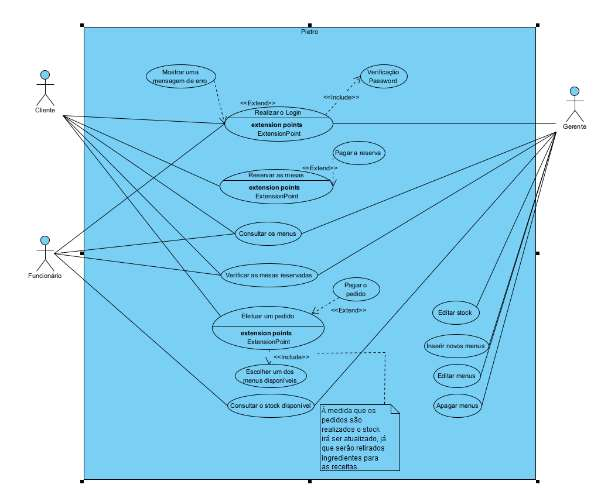
\includegraphics[width=14cm]{Resources/Previous/image-089.jpg}
    \caption{Diagrama de Casos de Uso (UML)}
    
\end{figure}

Quando o diagrama foi terminado, foram analisados os casos de uso e especificamos cada um deles. Para cada um dos casos de uso elaboramos uma breve descrição, definimos as pré e pós condições, o fluxo de eventos entre outras especificações.

De seguida são apresentadas as tabelas com as especificações para cada caso de uso.

\begin{figure}[!hbt]
    \centering
    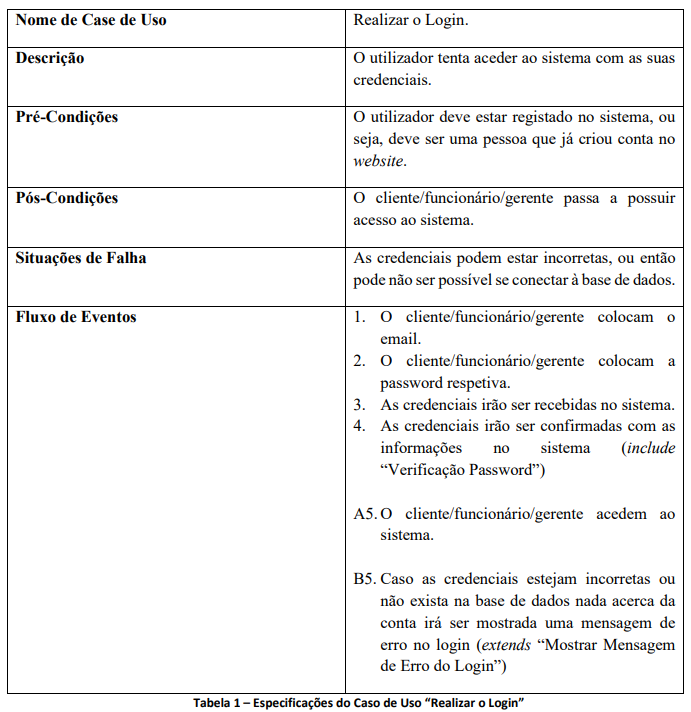
\includegraphics[width=14cm]{Resources/TablesPrintSc/1.png}
    \caption{PrintSc da Tabela 1}
    
\end{figure}
\FloatBarrier
\begin{figure}[!hbt]
    \centering
    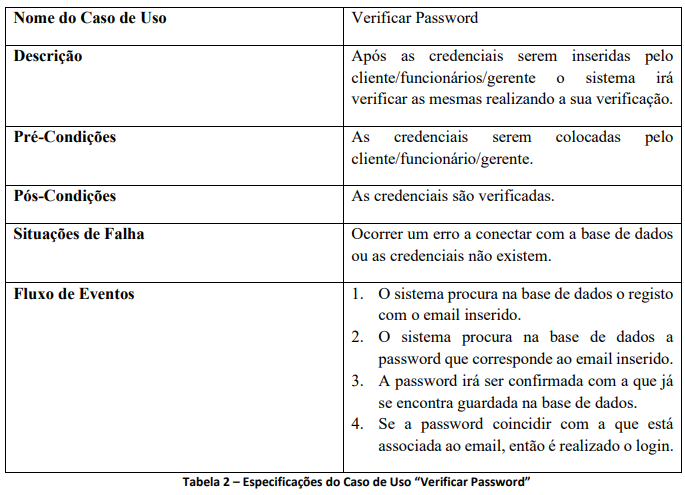
\includegraphics[width=14cm]{Resources/TablesPrintSc/2.png}
    \caption{PrintSc da Tabela 2}
    
\end{figure}
\FloatBarrier
\begin{figure}[!hbt]
    \centering
    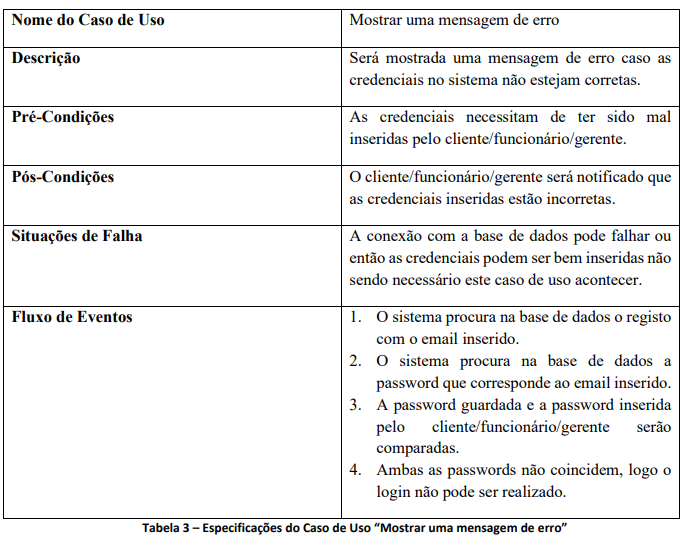
\includegraphics[width=14cm]{Resources/TablesPrintSc/3.png}
    \caption{PrintSc da Tabela 3}
    
\end{figure}
\FloatBarrier
\begin{figure}[!hbt]
    \centering
    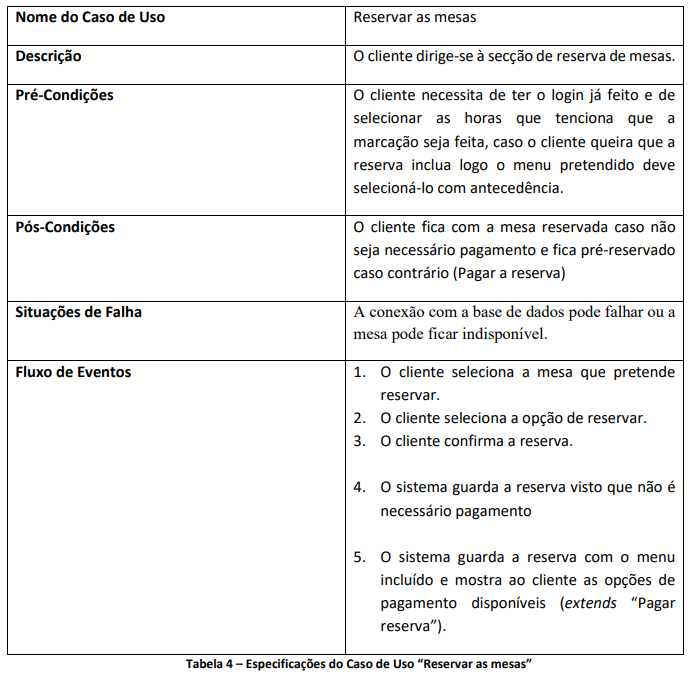
\includegraphics[width=14cm]{Resources/TablesPrintSc/4.png}
    \caption{PrintSc da Tabela 4}
    
\end{figure}
\FloatBarrier
\begin{figure}[!hbt]
    \centering
    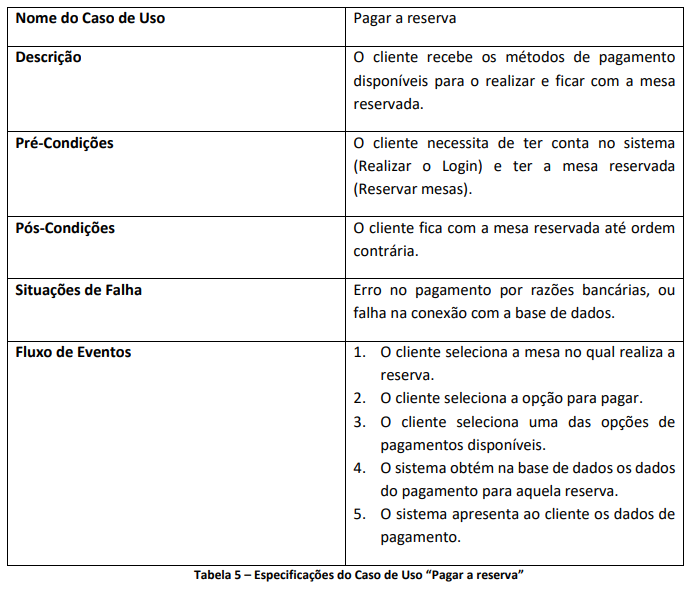
\includegraphics[width=14cm]{Resources/TablesPrintSc/5.png}
    \caption{PrintSc da Tabela 5}
    
\end{figure}
\FloatBarrier
\begin{figure}[!hbt]
    \centering
    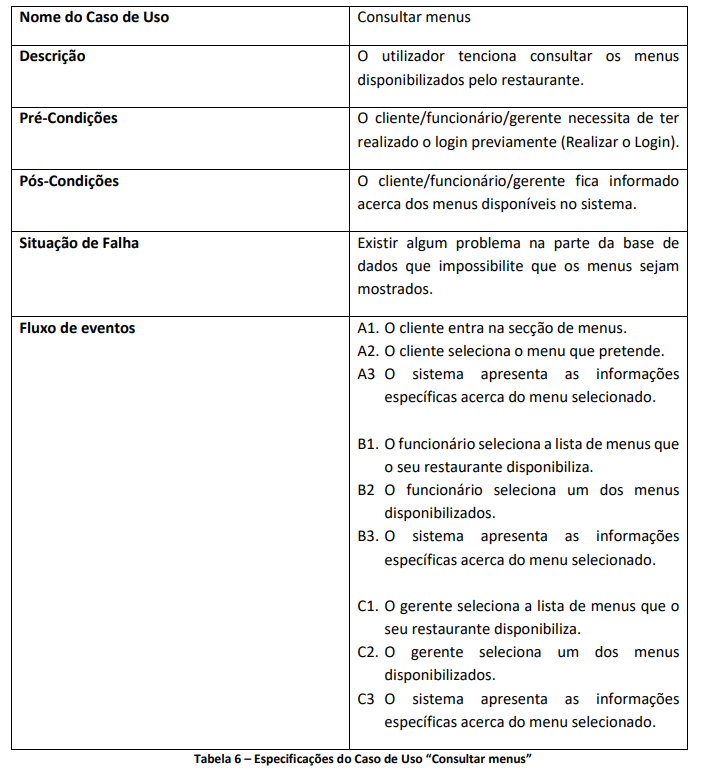
\includegraphics[width=14cm]{Resources/TablesPrintSc/6.png}
    \caption{PrintSc da Tabela 6}
    
\end{figure}
\FloatBarrier
\begin{figure}[!hbt]
    \centering
    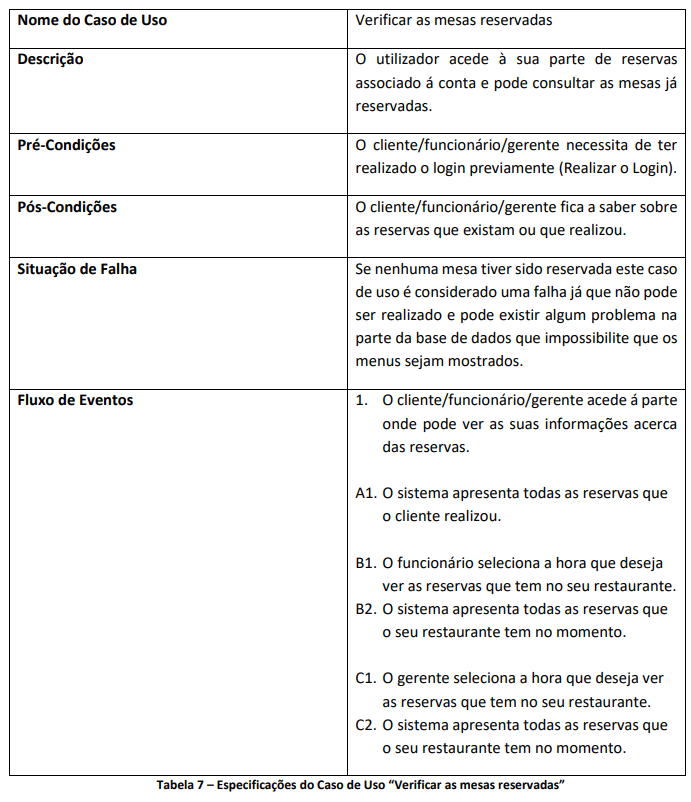
\includegraphics[width=14cm]{Resources/TablesPrintSc/7.png}
    \caption{PrintSc da Tabela 7}
    
\end{figure}
\FloatBarrier
\begin{figure}[!hbt]
    \centering
    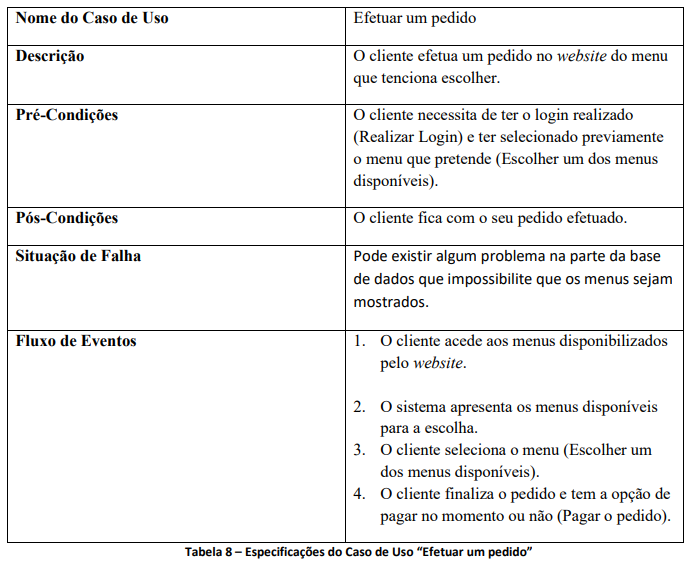
\includegraphics[width=14cm]{Resources/TablesPrintSc/8.png}
    \caption{PrintSc da Tabela 8}
    
\end{figure}
\FloatBarrier
\begin{figure}[!hbt]
    \centering
    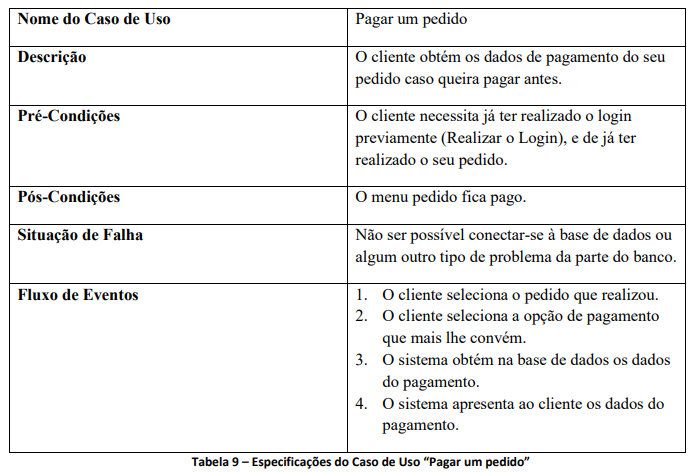
\includegraphics[width=14cm]{Resources/TablesPrintSc/9.png}
    \caption{PrintSc da Tabela 9}
    
\end{figure}
\FloatBarrier
\begin{figure}[!hbt]
    \centering
    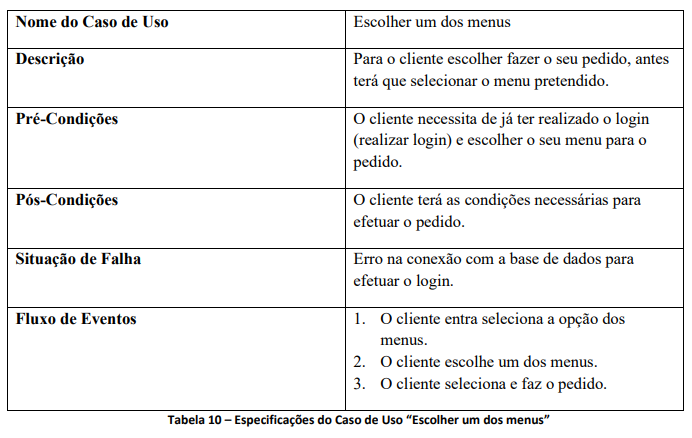
\includegraphics[width=14cm]{Resources/TablesPrintSc/10.png}
    \caption{PrintSc da Tabela 10}
    
\end{figure}
\FloatBarrier
\begin{figure}[!hbt]
    \centering
    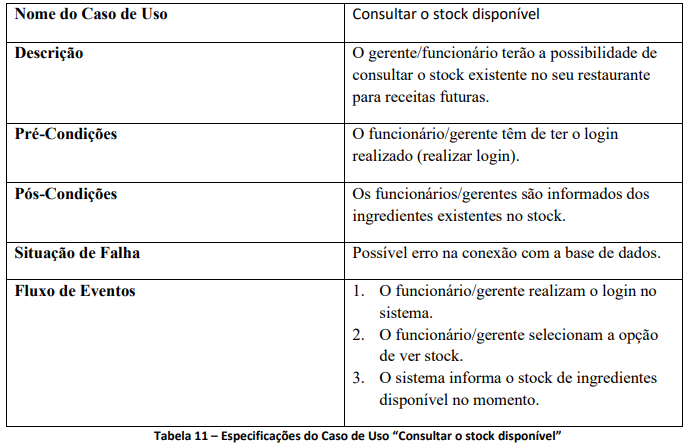
\includegraphics[width=14cm]{Resources/TablesPrintSc/11.png}
    \caption{PrintSc da Tabela 11}
    
\end{figure}
\FloatBarrier
\begin{figure}[!hbt]
    \centering
    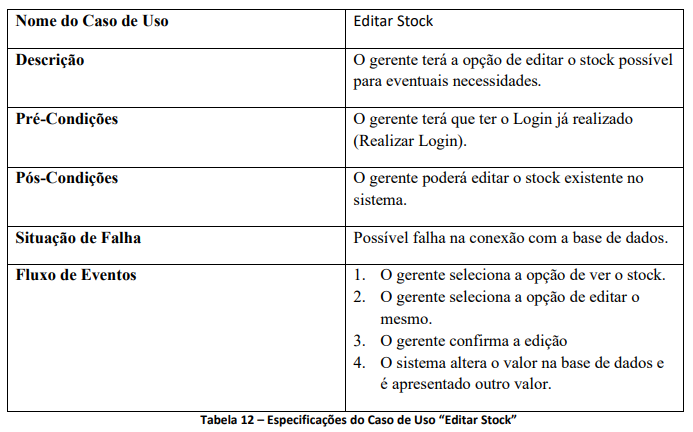
\includegraphics[width=14cm]{Resources/TablesPrintSc/12.png}
    \caption{PrintSc da Tabela 12}
    
\end{figure}
\FloatBarrier
\begin{figure}[!hbt]
    \centering
    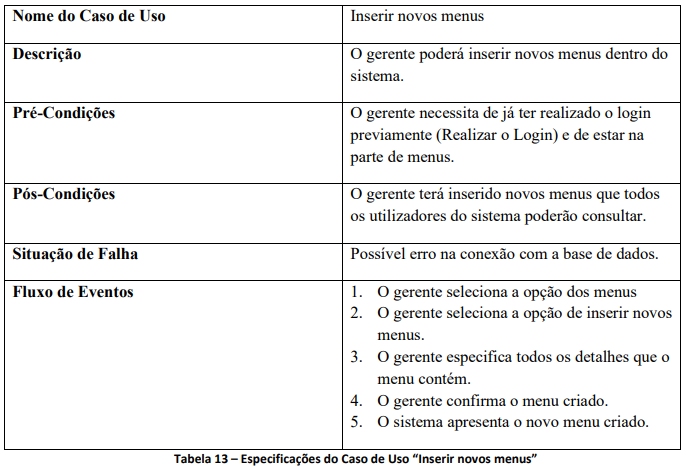
\includegraphics[width=14cm]{Resources/TablesPrintSc/13.png}
    \caption{PrintSc da Tabela 13}
    
\end{figure}
\FloatBarrier
\begin{figure}[!hbt]
    \centering
    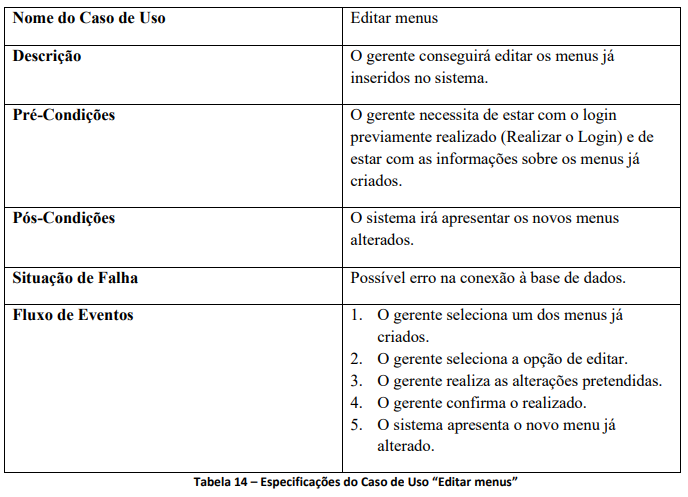
\includegraphics[width=14cm]{Resources/TablesPrintSc/14.png}
    \caption{PrintSc da Tabela 14}
    
\end{figure}
\FloatBarrier
\begin{figure}[!hbt]
    \centering
    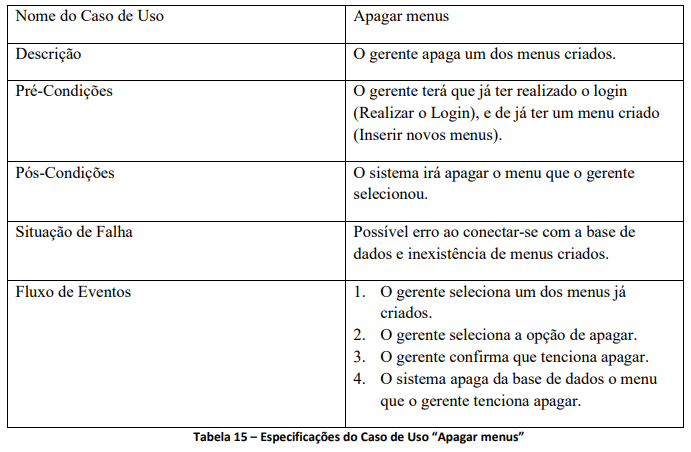
\includegraphics[width=14cm]{Resources/TablesPrintSc/15.png}
    \caption{PrintSc da Tabela 15}
    
\end{figure}
\FloatBarrier

\subsection{Desenho do Sistema}

O desenho inicial do protótipo foi realizado com o intuito de satisfazer todas as necessidades dos diferentes utilizadores na realização das tarefas já apresentadas. O objectivo do desenho foi ser o mais simples possível para que qualquer utilizador consiga utilizar o mesmo, o estilo de desenho que achamos por melhor utilizar foi o Flat Design, uma vez que é dos estilos mais modernos actualmente.


\begin{figure}[!hbt]
    \centering
    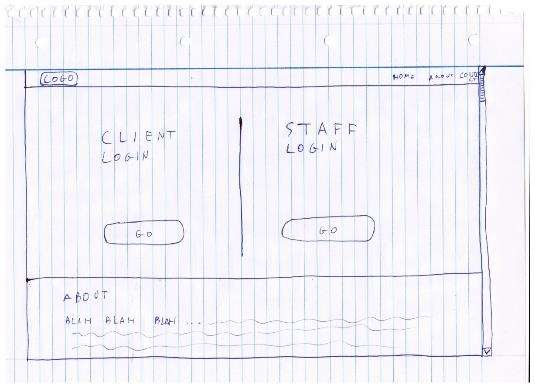
\includegraphics[width=14cm]{Resources/Previous/image-090.jpg}
    \caption{Desenho do Sistema 1}
    
\end{figure}
\FloatBarrier
\begin{figure}[!hbt]
    \centering
    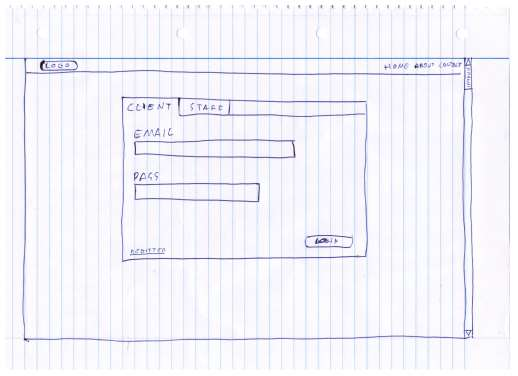
\includegraphics[width=14cm]{Resources/Previous/image-091.jpg}
    \caption{Desenho do Sistema 2}
    
\end{figure}
\FloatBarrier
\begin{figure}[!hbt]
    \centering
    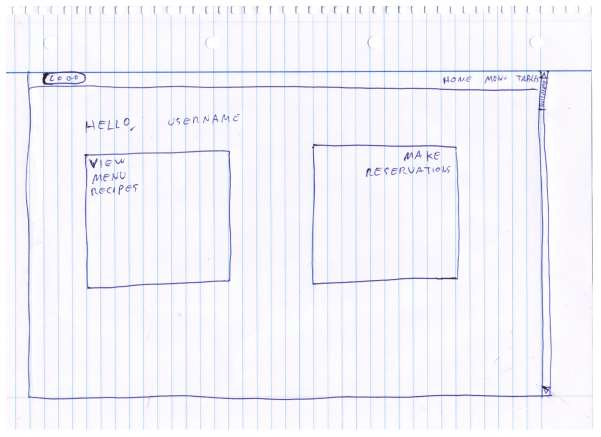
\includegraphics[width=14cm]{Resources/Previous/image-092.jpg}
    \caption{Desenho do Sistema 3}
    
\end{figure}
\FloatBarrier
\begin{figure}[!hbt]
    \centering
    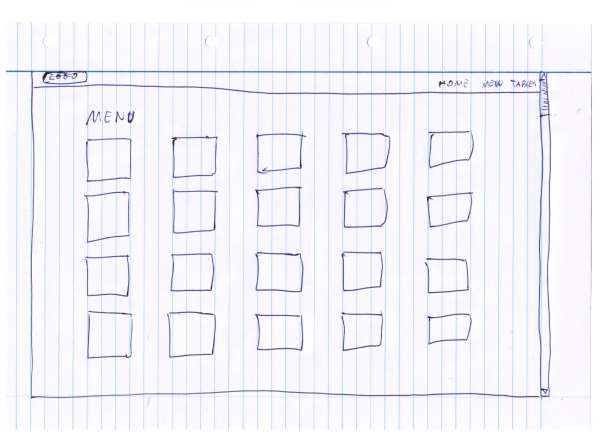
\includegraphics[width=14cm]{Resources/Previous/image-093.jpg}
    \caption{Desenho do Sistema 4}
    
\end{figure}
\FloatBarrier
\begin{figure}[!hbt]
    \centering
    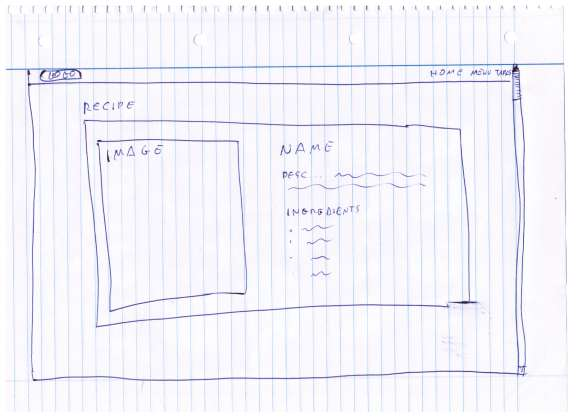
\includegraphics[width=14cm]{Resources/Previous/image-094.jpg}
    \caption{Desenho do Sistema 5}
    
\end{figure}
\FloatBarrier
\begin{figure}[!hbt]
    \centering
    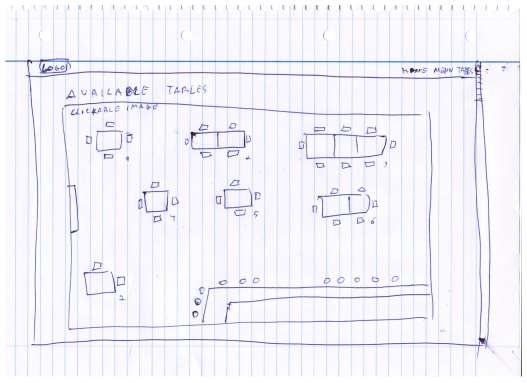
\includegraphics[width=14cm]{Resources/Previous/image-095.jpg}
    \caption{Desenho do Sistema 6}
    
\end{figure}
\FloatBarrier
\begin{figure}[!hbt]
    \centering
    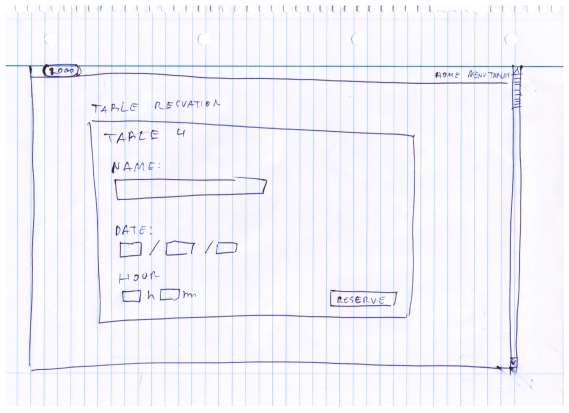
\includegraphics[width=14cm]{Resources/Previous/image-096.jpg}
    \caption{Desenho do Sistema 7}
    
\end{figure}
\FloatBarrier
\begin{figure}[!hbt]
    \centering
    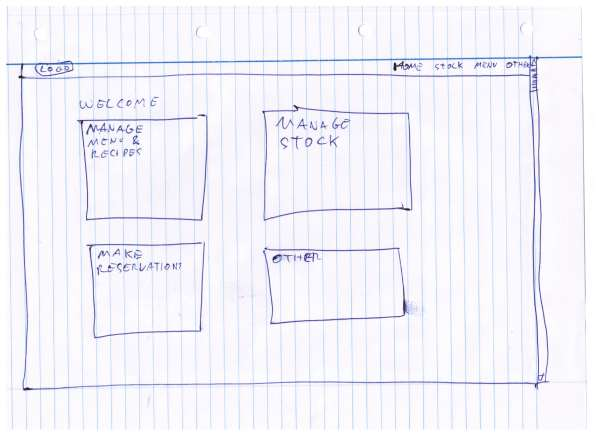
\includegraphics[width=14cm]{Resources/Previous/image-097.jpg}
    \caption{Desenho do Sistema 8}
    
\end{figure}
\FloatBarrier
\begin{figure}[!hbt]
    \centering
    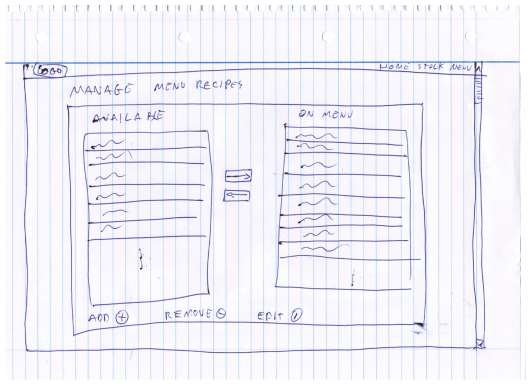
\includegraphics[width=14cm]{Resources/Previous/image-098.jpg}
    \caption{Desenho do Sistema 9}
    
\end{figure}
\FloatBarrier
\begin{figure}[!hbt]
    \centering
    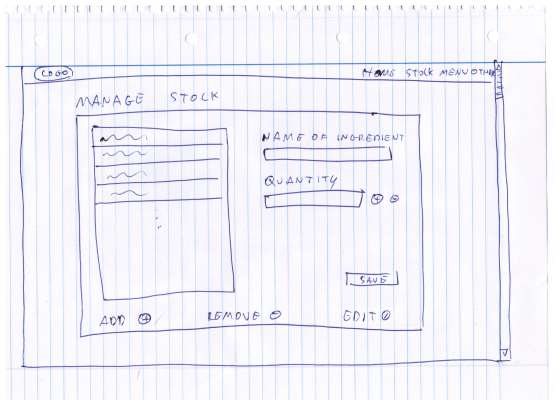
\includegraphics[width=14cm]{Resources/Previous/image-099.jpg}
    \caption{Desenho do Sistema 10}
    
\end{figure}
\FloatBarrier

\subsubsection{\textit{Storyboard}s}

Os \textit{Storyboard}s são desenhos sequenciais que pretendem ilustrar uma certa acção, é uma estratégia bastante útil uma vez que facilita o reconhecimento de erros e incongruências no desenho.

Em seguida são apresentados os \textit{Storyboard}s elaborados.

Caso de uso 1 (Gerir receitas. Adicionar, remover e editar as respectivas receitas de cada menu do cardápio).


\begin{figure}[!hbt]
    \centering
    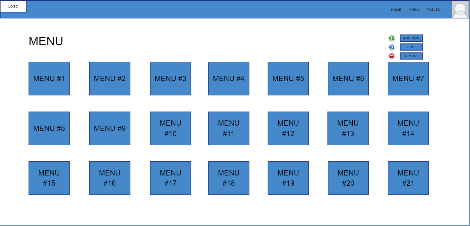
\includegraphics[width=14cm]{Resources/Previous/image-100.png}
    \caption{\textit{Storyboard} para o caso de uso 1}
    
\end{figure}
\FloatBarrier
\begin{figure}[!hbt]
    \centering
    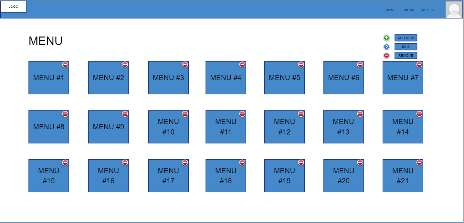
\includegraphics[width=14cm]{Resources/Previous/image-101.jpg}
    \caption{\textit{Storyboard} para o caso de uso 1}
    
\end{figure}
\FloatBarrier
\begin{figure}[!hbt]
    \centering
    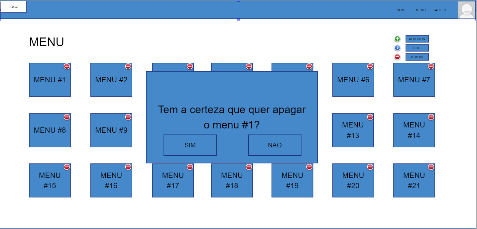
\includegraphics[width=14cm]{Resources/Previous/image-102.png}
    \caption{\textit{Storyboard} para o caso de uso 1}
    
\end{figure}
\FloatBarrier
\begin{figure}[!hbt]
    \centering
    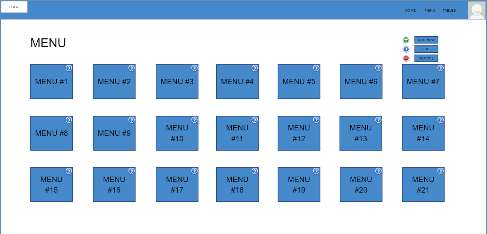
\includegraphics[width=14cm]{Resources/Previous/image-103.jpg}
    \caption{\textit{Storyboard} para o caso de uso 1}
    
\end{figure}
\FloatBarrier
\begin{figure}[!hbt]
    \centering
    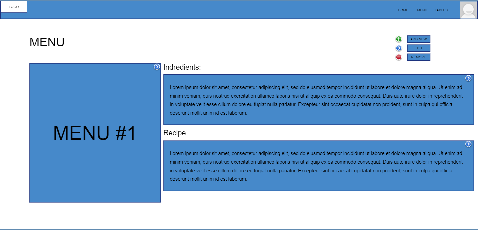
\includegraphics[width=14cm]{Resources/Previous/image-104.png}
    \caption{\textit{Storyboard} para o caso de uso 1}
    
\end{figure}
\FloatBarrier
\begin{figure}[!hbt]
    \centering
    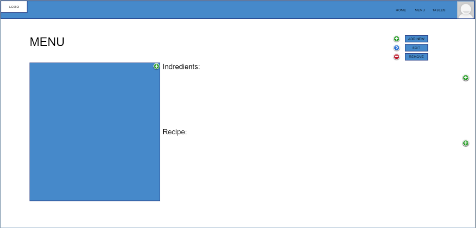
\includegraphics[width=14cm]{Resources/Previous/image-105.png}
    \caption{\textit{Storyboard} para o caso de uso 1}
    
\end{figure}
\FloatBarrier

Caso de uso 2 (Consulta das receitas. O cliente terá a opção de consultar as receitas disponíveis e os ingredientes que cada uma leva assim como alguns outros detalhes que poderão estar presentes.

\begin{figure}[!hbt]
    \centering
    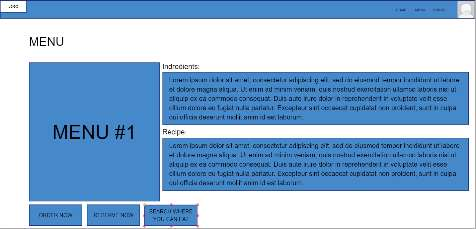
\includegraphics[width=14cm]{Resources/Previous/image-106.jpg}
    \caption{\textit{Storyboard} para o caso de uso 2}
    
\end{figure}
\FloatBarrier

Caso de uso 3 (Sistema de reservas (gerir mesas). Os clientes poderão ter a opção de entrar no sítio web para reservar uma mesa e os pratos que terão em mente.

Á medida que os clientes vão chegando e sentando-se nas devidas mesas, o sistema irá bloquear as mesas correspondentes às que estarão em uso e mais tarde serão desbloqueadas quando os clientes estiverem servidos).

\begin{figure}[!hbt]
    \centering
    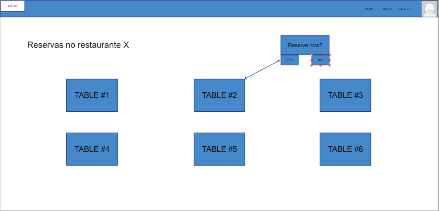
\includegraphics[width=14cm]{Resources/Previous/image-107.png}
    \caption{\textit{Storyboard} para o caso de uso 3}
    
\end{figure}
\FloatBarrier

Caso de uso 4 (Gerir o stock. Ao ser vendido um dos pratos do restaurante, será debitado do stock os ingredientes necessários para realizar a receita. Os funcionários poderão também consultar o stock existente no sistema).

\begin{figure}[!hbt]
    \centering
    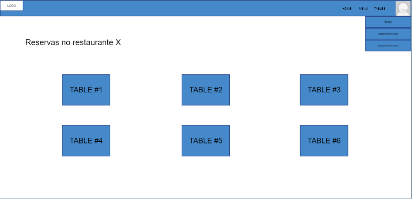
\includegraphics[width=14cm]{Resources/Previous/image-108.png}
    \caption{\textit{Storyboard} para o caso de uso 4}
    
\end{figure}
\FloatBarrier
\begin{figure}[!hbt]
    \centering
    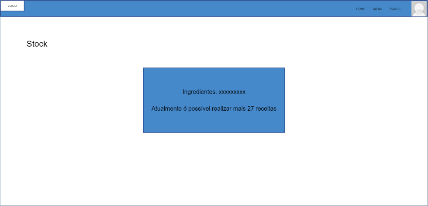
\includegraphics[width=14cm]{Resources/Previous/image-109.png}
    \caption{\textit{Storyboard} para o caso de uso 4}
    
\end{figure}
\FloatBarrier

\subsubsection{\textit{Drafts} das Interfaces 1 e 4}

\begin{figure}[!hbt]
    \centering
    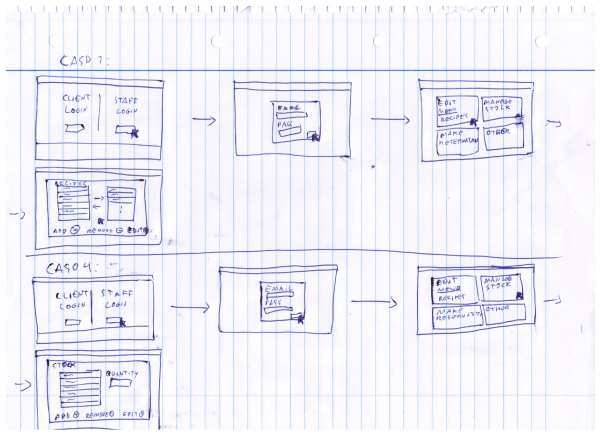
\includegraphics[width=14cm]{Resources/Previous/image-110.jpg}
    \caption{Interfaces para o caso de uso 1 e 4}
    
\end{figure}
\FloatBarrier


\subsubsection{\textit{Drafts} das Interfaces 2 e 3}

\begin{figure}[!hbt]
    \centering
    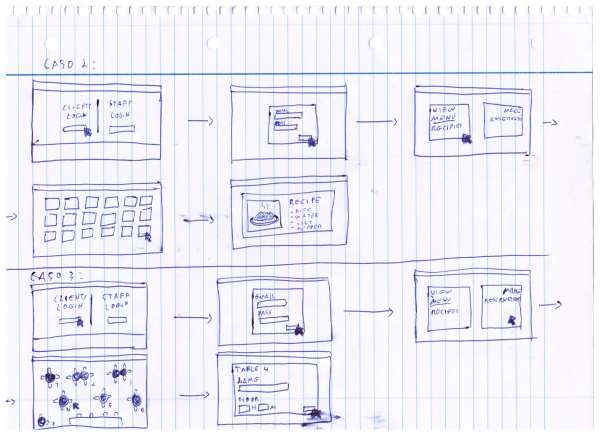
\includegraphics[width=14cm]{Resources/Previous/image-111.jpg}
    \caption{Interfaces para o caso de uso 2 e 3}
    
\end{figure}
\FloatBarrier

\subsection{Modelação da Base de Dados}

De modo que o sistema fosse capaz de armazenar toda a informação necessária, sem criar redundância, identificamos as entidades e as relações estritamente necessárias entre as mesmas no modelo ER. Posteriormente foi desenvolvido o modelo físico baseado no modelo ER.

As imagens dos modelos estão apresentadas logo abaixo.

\subsubsection{Diagrama de Entidade-Relação}

\begin{figure}[!hbt]
    \centering
    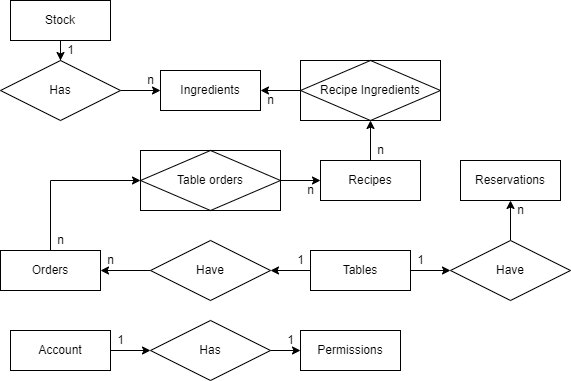
\includegraphics[width=14cm]{Resources/Previous/image-112.png}
    \caption{Diagrama ER}
    
\end{figure}
\FloatBarrier

\subsubsection{Modelo Físico}

\begin{figure}[!hbt]
    \centering
    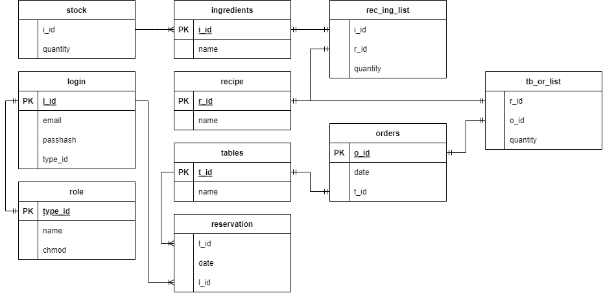
\includegraphics[width=14cm]{Resources/Previous/image-114.png}
    \caption{Modelo Físico}
    
\end{figure}
\FloatBarrier
\chapter{Inicio do Projecto}

O inicio do projecto começou com a criação de uma Base de Dados, que implementa o modelo definido no trabalho de investigação anterior, apresentado em época normal.

Seguidamente, foi criado um novo projecto no Visual Studio, que implementa o template de ASP.NET Core WebApp MVC, com a base de dados criada anteriormente.

Posteriormente foi inicializado um repositório git, em que definimos a origem para o meu repositório pessoal no GitHub, assim tendo uma portabilidade e gestão de versões.

Noto que para a aprendizagem e criação deste projecto, usei os tutoriais do \href{https:\/\/www.linkedin.com\/in\/nick-chapsas}{Nick Chapsas} \cite{nickLI} no \href{https:\/\/www.youtube.com\/c\/Elfocrash}{YouTube} \cite{nickYT} e o seus exemplos no \href{https:\/\/github.com\/Elfocrash}{GitHub} \cite{nickGH}.

\section{O Projecto}

Este projecto deve implementar um sistema de gestão de receitas, que deve permitir ao utilizador criar, editar e eliminar receitas.

Quer seja via web, ou via RESTful API.

\section{Estilo de código e estrutura do   projecto}

É o típico código OOP com estrutura MVC, com dois tipos de \textit{Models} um de Dados relacionados directamente com a Tabela da DB e um de Dados Transaccionais entre Cliente e Servidor, \textit{Views} e dois grupos de \textit{\textit{controllers}}, um de controlo interno para as \textit{Views} e outro de controlo externo para a API.

\subsection{Objectivos}

Visto que os dois casos de uso para mim escolhidos (dos quatro possíveis, estabelecidos no trabalho investigativo anterior), com suporte unânime do grupo\/par, foram:

\begin{itemize}
  \item \textbf{Consultar receitas e ingredients}: para consultar as receitas e os ingredients que estão associados a essas receitas.
  \item \textbf{Gestão de ingredientes e receitas}: para criar, editar ou eliminar ingredientes e receitas.
\end{itemize}

Conseguimos determinar que temos de facto, os quatro principais métodos HTTP (GET, POST, PUT, DELETE), os quais uma REST API usa (em conjunto com as tecnologias de notação JSON e XML) para comunicar.

Tendo assim uma boa base de estudo e trabalho prático.

Em suma, este trabalho tem de ser feito com o objectivo de aprender a usar a linguagem de programação ASP.NET Core, de forma a criar um sistema de gestão de receitas e ingredientes, com a possibilidade de criar, editar ou eliminar receitas e ingredientes via API RESTful e ainda com interface de gestão de receitas e ingredientes via Web.

\subsection{\textit{Models}}

O modelo de dados é um conjunto de classes que representam a estrutura de dados da aplicação.

Logo, os modelos principais são os da directoria \textit{Models}, que representam as tabelas da base de dados.

No entanto, existem também modelos que representam dados que não estão associados a uma tabela, mas sim servem para facilitar a utilização e comunicação nos controladores entre os clientes e o servidor.

Estes são os modelos da subdirectoria \textit{API}\/\textit{Models}, pois são modelos compostos, que são modelos que contêm dados de outros modelos, de forma a facilitar a comunicação entre cliente e servidor. São semelhantes a \textit{ViewModels}, melhor dizendo servem o mesmo propósito, mas atribuo outro nome visto que não estão relacionados com \textit{Views}.

Existem também \textit{ViewModel}, que como dito anteriormente com os seus similares, os compostos, servem para facilitar a comunicação entre cliente e servidor através de um modelo que facilite a criação de uma \textit{View}.

\subsection{\textit{Controllers}}

Um \textit{controller} é um conjunto de métodos que manipulam dados e são chamados pelo cliente.

Os controladores ``principais'' são os da directoria \textit{\textit{controllers}}, que representam os grupos de métodos que manipulam dados da aplicação de forma visual.

Ou seja, manipulam dados directamente para as \textit{Views} que eles geram.

Já para a API, os controladores são os da diretoria API\/\textit{\textit{controllers}}, que manipulam dados para a API (RESTful), em formato JSON, com a formatação referente ao modelo de dados composto.

\subsection{\textit{Views}}

As \textit{Views} são as páginas HTML que apresentam os dados para o cliente.

As \textit{Views} principais são as da directoria \textit{Views}, que representam as páginas HTML que apresentam dados para o cliente.

Estas são retornadas pelos controladores ``principais'', que são os controladores da directoria \textit{\textit{controllers}}, que manipulam dados para as \textit{Views}.

\chapter{Base de dados}

Como o approach foi decidido ser o Database First, criamos uma Base de Dados primeiro no SQL Server.

Para tal abrimos o SSMS e criamos uma Base de Dados com o mesmo nome do projecto, a qual abrimos uma Query onde listamos a estrutura e os dados iniciais.

\section{Notas}

A estrutura da base de dados foi a decidida anteriormente na analise de sistema, no então sofre umas alterações para que fosse possível a utilização do Entity Framework Core.

Estas alterações são o facto de todas as tabelas ter uma PK e qualquer FK tem de ter CASCADE (neste caso ON DELETE CASCADE).

\section{\textit{Query}}

\begin{lstlisting}[
    language=SQL,
    showspaces=false,
    basicstyle=\ttfamily,
    numbers=left,
    numberstyle=\tiny,
    commentstyle=\color{gray},
    breaklines=true
]

CREATE TABLE ingredients (i_id TINYINT PRIMARY KEY, name VARCHAR(32) NOT NULL);
CREATE TABLE tables (t_id TINYINT PRIMARY KEY, name VARCHAR(32) NOT NULL);
CREATE TABLE recipe (r_id TINYINT PRIMARY KEY, name VARCHAR(32) NOT NULL);
CREATE TABLE stock (
  i_id TINYINT PRIMARY KEY,
  quantity TINYINT NOT NULL,
  FOREIGN KEY (i_id) REFERENCES ingredients(i_id) ON DELETE CASCADE
);
CREATE TABLE rec_ing_list (
  ril_id TINYINT PRIMARY KEY,
  r_id TINYINT NOT NULL,
  i_id TINYINT NOT NULL,
  quantity TINYINT NOT NULL,
  FOREIGN KEY (r_id) REFERENCES recipe(r_id) ON DELETE CASCADE,
  FOREIGN KEY (i_id) REFERENCES ingredients(i_id) ON DELETE CASCADE
);
CREATE TABLE orders (
  o_id TINYINT PRIMARY KEY,
  date DATETIME NOT NULL,
  r_id TINYINT NOT NULL,
  FOREIGN KEY (r_id) REFERENCES recipe(r_id) ON DELETE CASCADE
);
CREATE TABLE tb_or_list (
  tol_id TINYINT PRIMARY KEY,
  o_id TINYINT NOT NULL,
  t_id TINYINT NOT NULL,
  quantity TINYINT NOT NULL,
  FOREIGN KEY (o_id) REFERENCES orders(o_id) ON DELETE CASCADE,
  FOREIGN KEY (t_id) REFERENCES tables(t_id) ON DELETE CASCADE
);
CREATE TABLE login_type (
  type_id TINYINT PRIMARY KEY,
  name VARCHAR(32) NOT NULL,
  chmod TINYINT NOT NULL
);
CREATE TABLE login (
  l_id TINYINT PRIMARY KEY,
  username VARCHAR(32) NOT NULL,
  passhash VARCHAR(32) NOT NULL,
  type_id TINYINT NOT NULL,
  FOREIGN KEY (type_id) REFERENCES login_type(type_id) ON DELETE CASCADE
);
CREATE TABLE reservation (
  res_id TINYINT PRIMARY KEY,
  t_id TINYINT NOT NULL,
  date DATETIME NOT NULL,
  l_id TINYINT NOT NULL,
  FOREIGN KEY (t_id) REFERENCES tables(t_id) ON DELETE CASCADE,
  FOREIGN KEY (l_id) REFERENCES login(l_id) ON DELETE CASCADE
);
INSERT INTO recipe (r_id, name)
VALUES (1, 'Cake'),
  (2, 'Cookie'),
  (3, 'Pancake'),
  (4, 'Pie');
INSERT INTO ingredients (i_id, name)
VALUES (1, 'Flour'),
  (2, 'Sugar'),
  (3, 'Eggs'),
  (4, 'Milk'),
  (5, 'Butter'),
  (6, 'Baking Powder'),
  (7, 'Salt'),
  (8, 'Vanilla'),
  (9, 'Cake Mix'),
  (10, 'Cookie Mix'),
  (11, 'Pancake Mix'),
  (12, 'Pie Mix');
INSERT INTO rec_ing_list (ril_id, r_id, i_id, quantity)
VALUES (1, 1, 1, 1),
  (2, 1, 2, 1),
  (3, 1, 3, 1),
  (4, 2, 4, 1),
  (5, 2, 5, 1),
  (6, 2, 6, 1),
  (7, 3, 7, 1),
  (8, 3, 8, 1),
  (9, 3, 9, 1),
  (10, 4, 10, 1),
  (11, 4, 11, 1),
  (12, 4, 12, 1);
INSERT INTO stock (i_id, quantity)
VALUES (1, 74),
  (2, 115),
  (3, 46),
  (4, 40),
  (5, 63),
  (6, 124),
  (7, 117),
  (8, 93),
  (9, 85),
  (10, 135),
  (11, 120),
  (12, 191);
INSERT INTO login_type (type_id, name, chmod)
VALUES (1, 'Admin', 1),
  (2, 'Manager', 2),
  (3, 'Employee', 3),
  (4, 'Customer', 4);
INSERT INTO login (l_id, username, passhash, type_id)
VALUES (1, 'admin', 'admin', 1),
  (2, 'manager', 'manager', 2),
  (3, 'employee', 'employee', 3),
  (4, 'customer', 'customer', 4);
INSERT INTO tables (t_id, name)
VALUES (1, 'Table 1'),
  (2, 'Table 2'),
  (3, 'Table 3'),
  (4, 'Table 4'),
  (5, 'Table 5'),
  (6, 'Table 6'),
  (7, 'Table 7'),
  (8, 'Table 8'),
  (9, 'Table 9'),
  (10, 'Table 10');
INSERT INTO reservation (res_id, t_id, date, l_id)
VALUES (1, 6, '2022-01-17 17:00:00', 1),
  (2, 7, '2022-01-17 18:30:0', 1),
  (3, 8, '2022-01-17 19:30:00', 1),
  (4, 9, '2022-01-18 13:00:00', 1),
  (5, 10, '2022-01-19 12:30:00', 1);
INSERT INTO orders (o_id, date, r_id)
VALUES (1, '2022-01-17 17:00:00', 1),
  (2, '2022-01-17 18:30:0', 1),
  (3, '2022-01-17 19:30:00', 1),
  (4, '2022-01-18 13:00:00', 1),
  (5, '2022-01-19 12:30:00', 1);
INSERT INTO tb_or_list (tol_id, o_id, t_id, quantity)
VALUES (1, 1, 6, 1),
  (2, 2, 7, 1),
  (3, 3, 8, 1),
  (4, 4, 9, 1),
  (5, 5, 10, 1);

\end{lstlisting}

\newpage
\section{Conteúdo Gerado}

A \textit{Query} no final da execução gerou a base de dados com a seguinte estrutura:

\begin{figure}[!hbt]
    \centering
    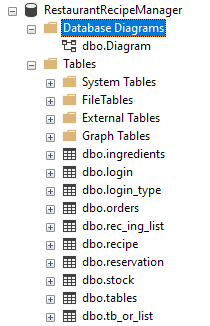
\includegraphics[width=6cm]{Resources/Database/DB (2).png}
    \caption{Tabelas Geradas}
    
\end{figure}

A qual melhor demonstrada via este Diagrama:

\begin{figure}[!hbt]
    \centering
    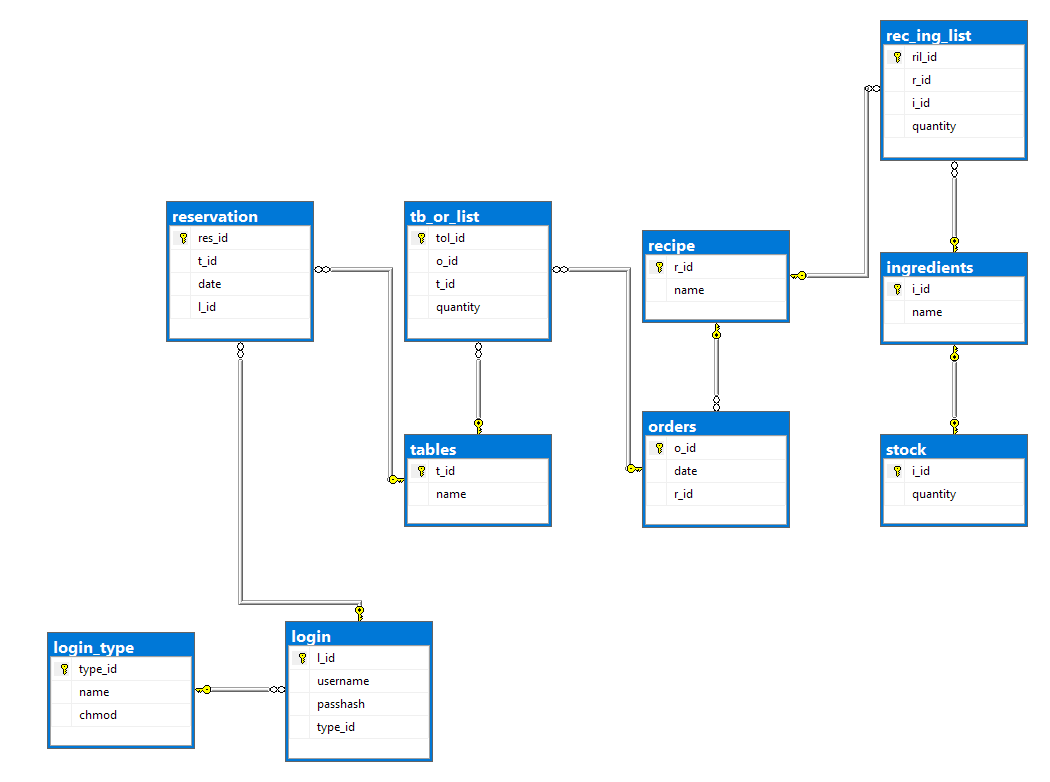
\includegraphics[width=14cm]{Resources/Database/DB (1).png}
    \caption{Diagrama da base de dados}
    
\end{figure}
\chapter{Implementação da API}

A API RESTful para comunicação externa foi a primeira tarefa a ser desenvolvida.

A sua conclusão delinearia a estrutura do projecto e encaminhava a forma como os dados são tratados e como os reimplementamos nos controladores com \textit{Views}.

Para uma API ser RESTful, deve ser possível a comunicação entre o cliente e o servidor, via os métodos HTTP (GET, POST, PUT, DELETE, etc, e com a formatação referente ao modelo de dados num formato de notação de objectos (JSON ou XML).

Esta deve também usar um \textit{standard} de nomenclatura para comunicar os erros.

Esse \textit{standard} usa cinco trios de números, dos quais os que começam por 1 são mensagens informativas, os que começam por 2 são mensagens de sucesso, os que começam por 3 são mensagens de redireccionamento, os que começam por 4 são mensagens de erro de cliente e os que começam por 5 são mensagens de erro de servidor.

Neste caso específico, a API RESTful usa o modelo de dados composto, semelhante a um \textit{ViewModel}, que é um modelo de dados que contém dados de outros modelos, em formato de notação JSON, para via os quatro principais métodos HTTP (GET, POST, PUT, DELETE).

\section{Gestão de ingredientes}

Para a gestão de ingredientes, a API RESTful usa dois métodos HTTP GET, um POST, um PUT e um DELETE.

Os quais são usados para consultar todos os ingredientes, consultar um ingrediente específico, criar um ingrediente, editar um ingrediente ou eliminar um ingrediente.

Estes URI são:

\begin{itemize}
  \item \textit{/api/ingredients/list}: \textbf{GET} para consultar todos os ingredientes.
  \item \textit{/api/ingredients/view/\{id\}}: \textbf{GET} para consultar um ingrediente específico.
  \item \textit{/api/ingredients/add}: \textbf{POST} para criar um ingrediente. Usamos no \textit{body} no formato JSON para enviar os dados, com o formato do IngredienteModel (que é um modelo composto).
  \item \textit{/api/ingredients/edit/}: \textbf{PUT} para editar um ingrediente. Usamos no \textit{body} no formato JSON para enviar os dados, com o formato do IngredienteModel (que é um modelo composto).
  \item \textit{/api/ingredients/remove/\{id\}}: \textbf{DELETE} para eliminar um ingrediente.
\end{itemize}

O modelo de dados composto, IngredientModel, contém os seguintes
campos:

\begin{itemize}
  \item \textbf{IId}: identificador do ingrediente.
  \item \textbf{Name}: nome do ingrediente.
  \item \textbf{Quantity}: quantidade do ingrediente.
\end{itemize}

Estes campos são obrigatórios.

\section{Gestão de receitas}

Na gestão de receitas, a API RESTful usa dois métodos HTTP GET, um POST, um PUT e um DELETE.

Os quais são usados para consultar todas as receitas, consultar uma receita específica, criar uma receita, editar uma receita ou eliminar uma receita.

Os URI são:

\begin{itemize}
  \item \textit{/api/recipes/list}: \textbf{GET} para consultar todas as receitas.
  \item \textit{/api/recipes/view/\{id\}}: \textbf{GET} para consultar uma receita específica.
  \item \textit{/api/recipes/add}: \textbf{POST} para criar uma receita. Usamos no \textit{body} no formato JSON para enviar os dados, com o formato do RecipeModel (que é um modelo composto).
  \item \textit{/api/recipes/edit/}: \textbf{PUT} para editar uma receita. Usamos no \textit{body} no formato JSON para enviar os dados, com o formato do RecipeModel (que é um modelo composto).
  \item \textit{/api/recipes/remove/\{id\}}: \textbf{DELETE} para eliminar uma receita.
\end{itemize}

O RecipeModel, que é um modelo composto, contém os seguintes campos:

\begin{itemize}
  \item \textbf{RId}: identificador da receita.
  \item \textbf{Name}: nome da receita.
  \item \textbf{Ingredients}: ingredientes da receita.
\end{itemize}

Este campo Ingredients é um IEnumerable, que é um tipo de dados que permite a criação de listas de dados.

Esta lista é composta por objectos do tipo RecipeModel.Ingredient, que é um objecto interno do modelo RecipeModel.

Este objeto é composto pelos seguintes campos:

\begin{itemize}
  \item \textbf{IId}: identificador do ingrediente.
  \item \textbf{Quantity}: quantidade do ingrediente.
\end{itemize}
\section{Error Handling}

Para a gestão de erros, a API está rodeada de blocos \textit{try-catch} e faz vários \textit{checks if} para verificar se ocorreu algum erro.

Se ocorreu, o erro é tratado e retornado ao cliente um código de erro e uma mensagem de erro.

Os códigos de erro são:

\begin{itemize}
  \item \textbf{400}: Bad Request. Ocorre quando o cliente envia dados mal formatados.
  \item \textbf{404}: \textit{Not Found}. Ocorre quando o recurso não foi encontrado.
  \item \textbf{500}: \textit{Internal Server Error}. Ocorre quando ocorre um erro no servidor.
\end{itemize}

Na versão rescrita da API, como existe o uso de um login básico
(inseguro, mas funcional) com nome e hash no \textit{body}, a API pode
ainda retornar:

\begin{itemize}
  \item \textbf{401}: \textit{Unauthorized}. Ocorre quando o cliente não está autenticado.
  \item \textbf{403}: \textit{Forbidden}. Ocorre quando o cliente não tem permissão para aceder ao recurso.
\end{itemize}

\section{Implementação de uma Autenticação (básica e
  insegura)}

Foi criada uma classe privada herdeira do modelo composto adequado ao controlador, onde se adiciona o campo \textit{UserName} e \textit{Passhash}. Estes campos são usados para autenticar o cliente.

A qual vamos buscar a role do usuário se o mesmo estiver autenticado, para verificar se o cliente tem permissão para aceder ao recurso.

Esta verificação é feita no método inicio do método responsável por executar a acção pedida, onde retorna o código de erro 403 (\textit{Forbidden}) se o cliente não tiver permissão para aceder ao recurso, ou o código de erro 401 (\textit{Unauthorized}) se o cliente não estiver autenticado ou a hash não corresponder à hash do utilizador.

\chapter{Implementação da Aplicação Web}

A aplicação web é constituída por um conjunto de páginas HTML, que são carregadas pelo servidor. Estas usam um roteamento diferente, que é na prática uma API interna, que é acessada pelo cliente através dos formulários nas \textit{Views}.

\section{Gestão de ingredientes}

Para a gestão de ingredientes, a Webapp usa quatro métodos HTTP GET e dois métodos HTTP POST. Os quais são usados para consultar todos os ingredientes, consultar um ingrediente específico, criar um ingrediente e editar um ingrediente. Não existe a utilização de métodos PUT e DELETE, visto que os formulários HTML e Razor não suportam estes métodos.

Estes URI são:

\begin{itemize}
  \item \textit{/api/ingredient/all}: \textbf{GET} para consultar todos os
  ingredientes.
  \item \textit{/api/ingredient/view/\{id\}}: \textbf{GET} para consultar um
  ingrediente específico.
  \item \textit{/api/ingredient/add}: \textbf{GET} para receber o formulário
  para criar um ingrediente.
  \item \textit{/api/ingredient/edit/\{id\}}: \textbf{GET} para receber o
  formulário para editar um ingrediente.
  \item \textit{/api/ingredient/delete/\{id\}}: \textbf{GET} para eliminar um
  ingrediente.
\end{itemize}

Os quais comunicam com as URI:

\begin{itemize}
  \item \textit{/api/ingredient/applyadd}: \textbf{POST} para criar um
  ingrediente.
  \item \textit{/api/ingredient/applyedit}: \textbf{POST} para editar um
  ingrediente.
\end{itemize}

O modelo de dados composto, IngredienteModel, contém os seguintes
campos:

\begin{itemize}
  \item \textbf{IId}: identificador do ingrediente.
  \item \textbf{Name}: nome do ingrediente.
  \item \textbf{Quantity}: quantidade do ingrediente.
\end{itemize}

Estes campos são obrigatórios.

\section{Gestão de receitas}

Na gestão de receitas, a API RESTful usa sete métodos HTTP GET e quatro métodos HTTP POST. Os quais são usados para consultar todas as receitas, consultar uma receita específica, criar uma receita e editar uma receita. Não existe a utilização de métodos PUT e DELETE, visto que os formulários HTML e Razor não suportam estes métodos.

Os URI são:

\begin{itemize}
  \item \textit{/api/recipe/all}: \textbf{GET} para consultar todas as receitas.
  \item \textit{/api/recipe/view/\{id\}}: \textbf{GET} para consultar uma
  receita específica.
  \item \textit{/api/recipe/add}: \textbf{GET} para receber o formulário para
  criar uma receita.
  \item \textit{/api/recipe/addingredient/\{id\}}: \textbf{GET} para receber o
  formulário para adicionar um ingrediente à receita.
  \item \textit{/api/recipe/editname/\{id\}}: \textbf{GET} para receber o
  formulário para editar o nome de uma receita.
  \item \textit{/api/recipe/editingredients/\{id\}}: \textbf{GET} para receber o
  formulário para ver os ingredientes a editar de uma receita.
  \item \textit{/api/recipe/editingredient/\{id\}}: \textbf{GET} para receber o
  formulário para editar um ingrediente de uma receita.
  \item \textit{/api/recipe/delete/\{id\}}: \textbf{GET} para eliminar uma
  receita.
  \item \textit{/api/recipe/deleteingredient/\{id\}}: \textbf{GET} para eliminar
  um ingrediente de uma receita.
\end{itemize}

Os quais comunicam com as URI:

\begin{itemize}
  \item \textit{/api/recipe/applyadd}: \textbf{POST} para criar uma receita.
  \item \textit{/api/recipe/applyaddingredient}: \textbf{POST} para adicionar um
  ingrediente à receita.
  \item \textit{/api/recipe/applynameedit}: \textbf{POST} para editar o nome de
  uma receita.
  \item \textit{/api/recipe/applyingredientedit}: \textbf{POST} para editar um
  ingrediente de uma receita.
\end{itemize}

O RecipeVM, que é um \textit{ViewModel}, contém os seguintes campos:

\begin{itemize}
  \item \textbf{RId}: identificador da receita.
  \item \textbf{Name}: nome da receita.
\end{itemize}

O RecipeAddVM, que é um \textit{ViewModel}, contém os seguintes campos:

\begin{itemize}
  \item \textbf{RId}: identificador da receita.
  \item \textbf{RilId}: identificador do ingrediente-receita.
  \item \textbf{IId}: identificador do ingrediente.
  \item \textbf{Name}: nome da receita.
  \item \textbf{Quantity}: quantidade do ingrediente.
\end{itemize}

O RecIngListsVM, que é um \textit{ViewModel}, contém os seguintes campos:

\begin{itemize}
  \item \textbf{RId}: identificador da receita.
  \item \textbf{IId}: identificador do ingrediente.
  \item \textbf{RilId}: identificador do ingrediente-receita.
  \item \textbf{Quantity}: quantidade do ingrediente.
\end{itemize}


\section{Error Handling}

Para a gestão de erros, a API está rodeada de blocos \textit{try-catch} e faz vários \textit{checks if} para verificar se ocorreu algum erro. Se ocorreu, o erro é tratado e retornado ao cliente um código de erro e uma mensagem de erro.

Os códigos de erro são:

\begin{itemize}
  \item \textbf{400}: Bad Request. Ocorre quando o cliente envia dados mal
  formatados.
  \item \textbf{404}: Not Found. Ocorre quando o recurso não foi encontrado.
  \item \textbf{500}: Internal Server Error. Ocorre quando ocorre um erro no
  servidor.
\end{itemize}

Na versão rescrita da API, como existe o uso de um login básico (inseguro, mas funcional) com nome e hash no \textit{body}, a API pode ainda retornar:

\begin{itemize}
  \item \textbf{401}: Unauthorized. Ocorre quando o cliente não está
  autenticado.
  \item \textbf{403}: Forbidden. Ocorre quando o cliente não tem permissão
  para aceder ao recurso.
\end{itemize}

\chapter{Teste do Projecto}

Aqui demonstro o funcionamento do projecto, via testes a duas secções: a API e a interface. Para esta demonstração em cada uma das secções, vamos utilizar imagens representativas, tiradas através de \textit{PrintScreen}.

Qualquer teste começa sempre pelo \textit{Home} (o \textit{Index}).

\begin{figure}[!hbt]
    \centering
    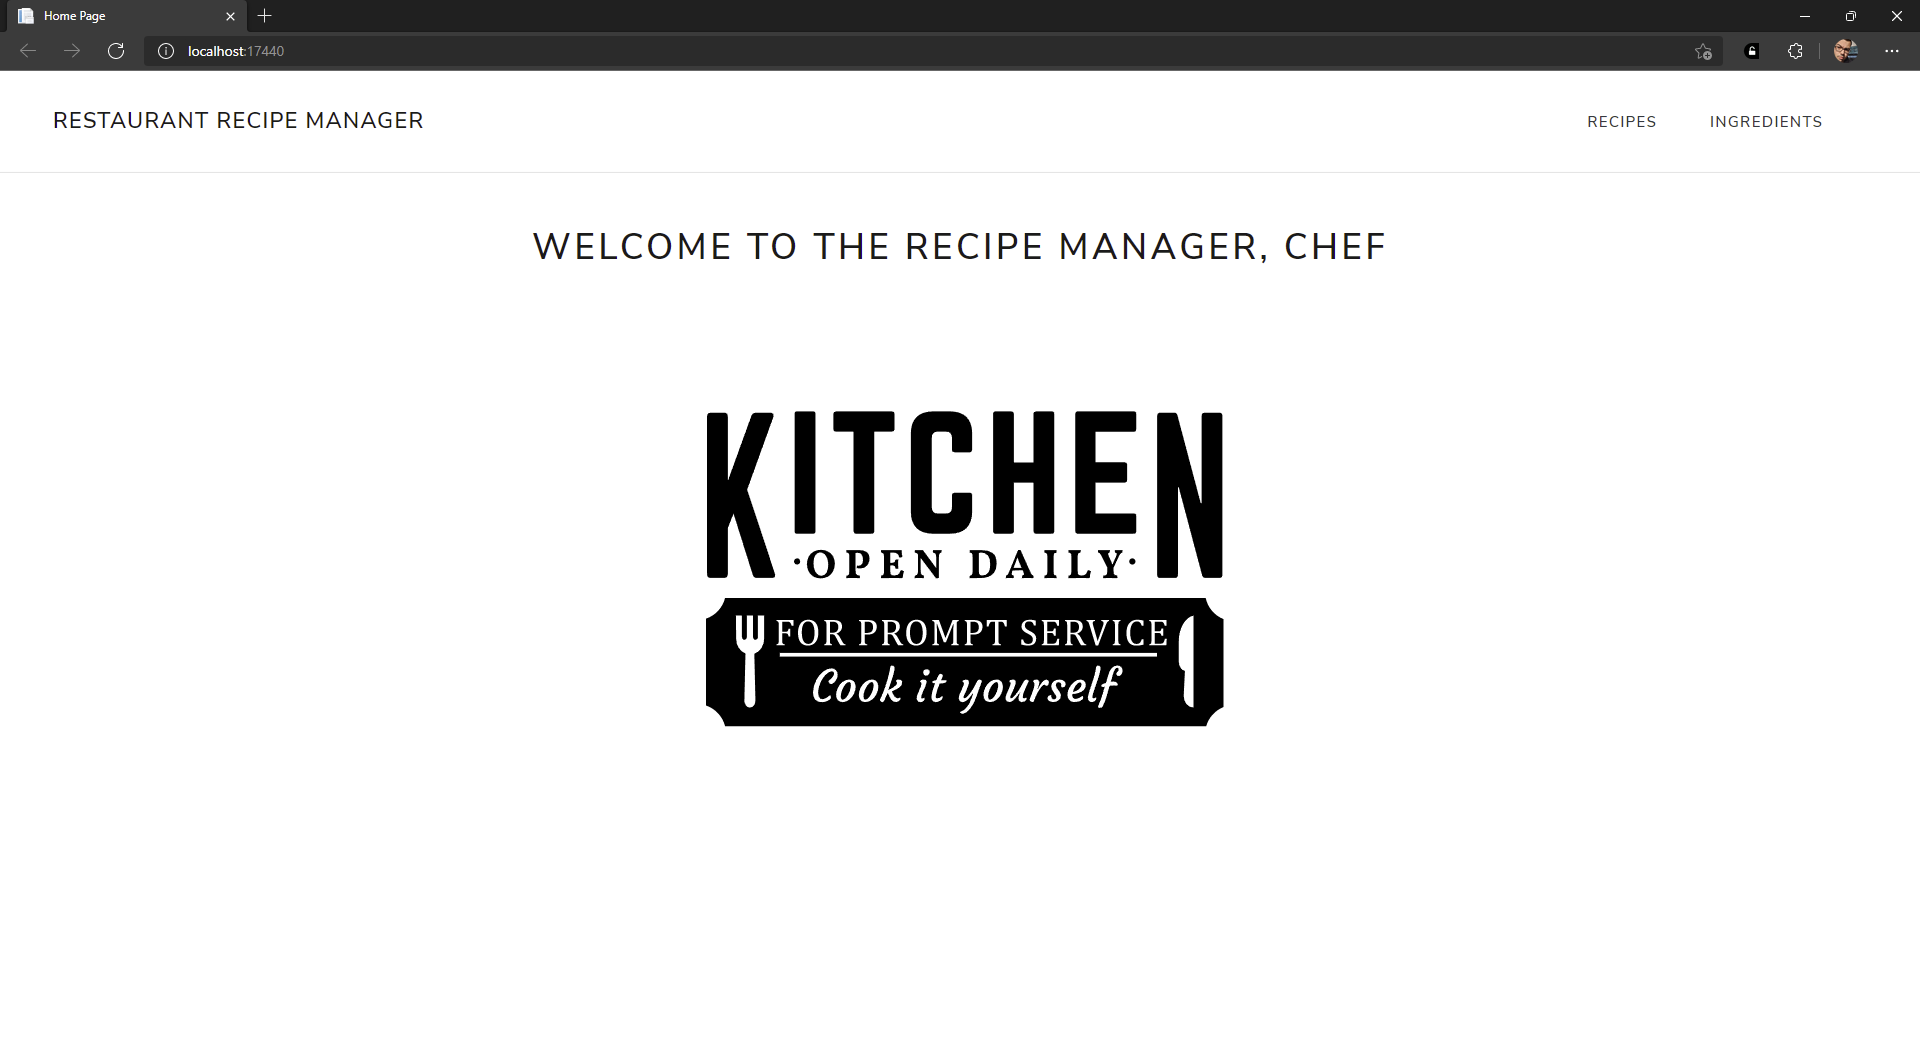
\includegraphics[width=14cm]{Resources/WebApp/Home/home.png}
    \caption{Ilustração do home da WebApp}
    \label{fig:home}
\end{figure}
\FloatBarrier

\section{Testes à API}

Para testar a API foi usado a extensão \textit{Thunder Client} do \textit{Visual Studio Code}. Esta é uma extensão que substitui o \textit{Postman}, que é um cliente HTTP que permite testar APIs.

Nas imagens seguintes podemos ver a API em funcionamento. O primeiro \textit{set} de imagens é referente ao caso de uso da Gestão de Ingredientes e Stock. O segundo referente ao caso de uso da Gestão de Receitas.

\newpage
\subsection{\textit{API/Ingredients}}

\begin{figure}[!hbt]
    \centering
    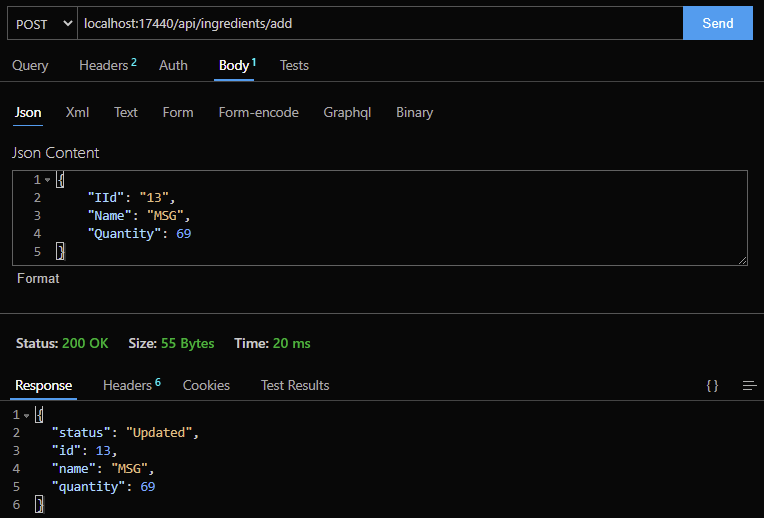
\includegraphics[width=14cm]{Resources/API/Ingredients/Ingredients (1).png}
    \caption{Ilustração do método POST a \textit{/api/ingredients/add}}
    \label{fig:api_ing_1}
\end{figure}
\FloatBarrier
\begin{figure}[!hbt]
    \centering
    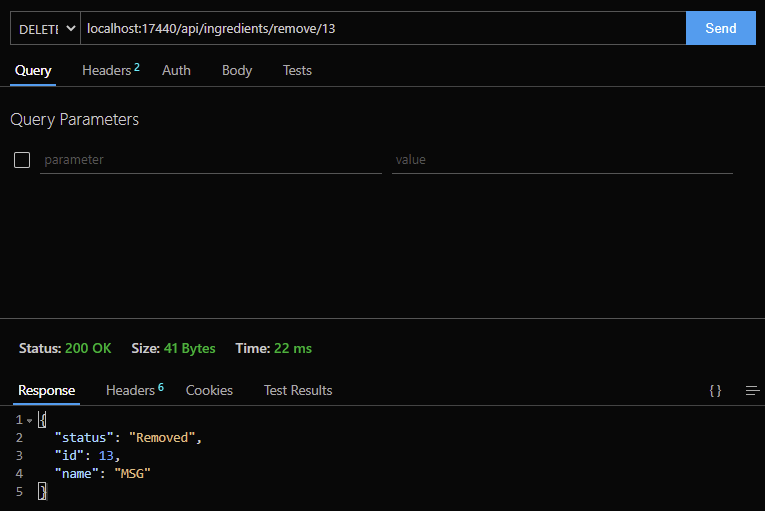
\includegraphics[width=14cm]{Resources/API/Ingredients/Ingredients (2).png}
    \caption{Ilustração do método DELETE a \textit{/api/remove/13}}
    \label{fig:api_ing_2}
\end{figure}
\FloatBarrier
\begin{figure}[!hbt]
    \centering
    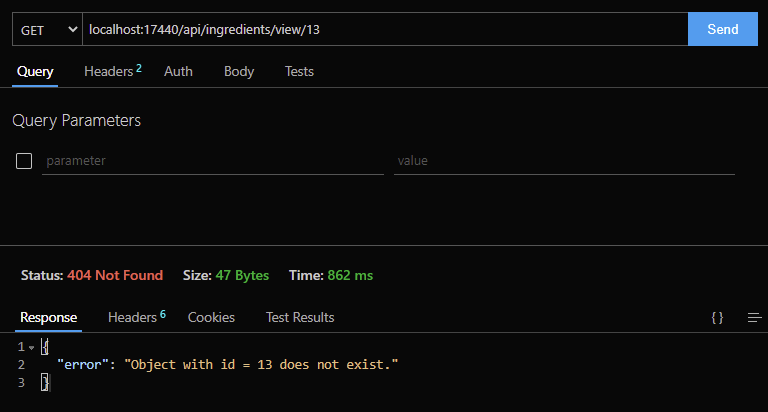
\includegraphics[width=14cm]{Resources/API/Ingredients/Ingredients (3).png}
    \caption{Ilustração do método GET a \textit{/api/ingredients/view/13}}
    \label{fig:api_ing_3}
\end{figure}
\FloatBarrier
\begin{figure}[!hbt]
    \centering
    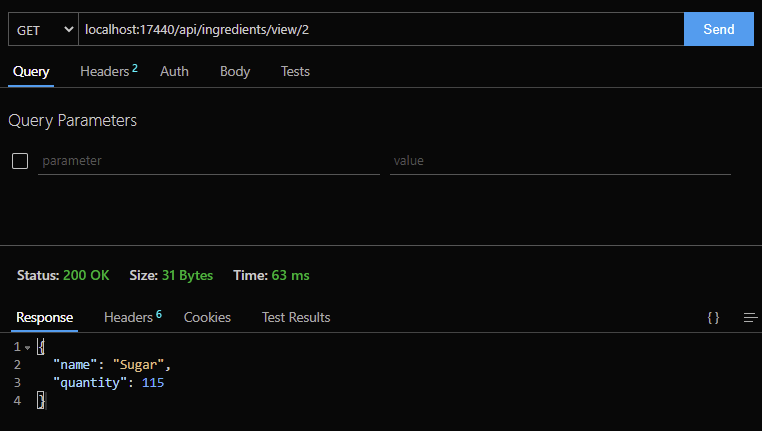
\includegraphics[width=14cm]{Resources/API/Ingredients/Ingredients (4).png}
    \caption{Ilustração do método GET a \textit{/api/ingredients/view/2}}
    \label{fig:api_ing_4}
\end{figure}
\FloatBarrier
\begin{figure}[!hbt]
    \centering
    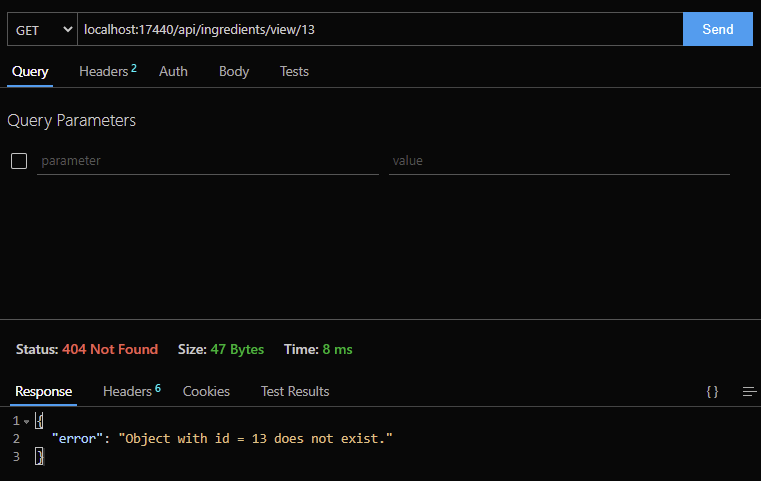
\includegraphics[width=14cm]{Resources/API/Ingredients/Ingredients (5).png}
    \caption{Ilustração do método GET a \textit{/api/ingredients/view/13}}
    \label{fig:api_ing_5}
\end{figure}
\FloatBarrier
\begin{figure}[!hbt]
    \centering
    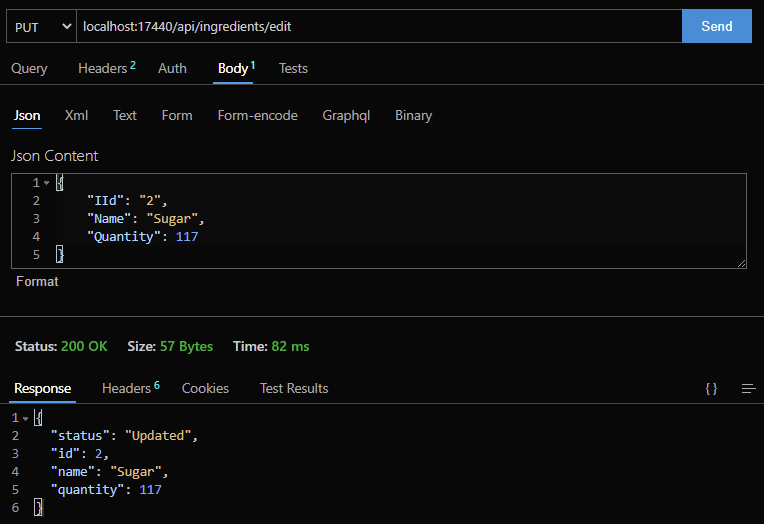
\includegraphics[width=14cm]{Resources/API/Ingredients/Ingredients (6).png}
    \caption{Ilustração do método PUT a \textit{/api/ingredients/edit}}
    \label{fig:api_ing_6}
\end{figure}
\FloatBarrier
\begin{figure}[!hbt]
    \centering
    \includegraphics[width=14cm]{Resources/API/Ingredients/Ingredients (7).png}
    \caption{Ilustração do método GET a \textit{/api/ingredients/list}}
    \label{fig:api_ing_7}
\end{figure}
\FloatBarrier
\begin{figure}[!hbt]
    \centering
    \includegraphics[width=14cm]{Resources/API/Ingredients/Ingredients (8).png}
    \caption{Ilustração do método GET a \textit{/api/ingredients/view/2}}
    \label{fig:api_ing_8}
\end{figure}
\FloatBarrier

\newpage
\subsection{\textit{API/Recipes}}

\begin{figure}[!hbt]
    \centering
    \includegraphics[width=14cm]{Resources/API/Recipes/Recipes (1).png}
    \caption{Ilustração do método GET a \textit{/api/recipes/view/5}}
    \label{fig:api_rec_1}
\end{figure}
\FloatBarrier
\begin{figure}[!hbt]
    \centering
    \includegraphics[width=14cm]{Resources/API/Recipes/Recipes (2).png}
    \caption{Ilustração do método POST a \textit{/api/recipes/add}}
    \label{fig:api_rec_2}
\end{figure}
\FloatBarrier
\begin{figure}[!hbt]
    \centering
    \includegraphics[width=14cm]{Resources/API/Recipes/Recipes (3).png}
    \caption{Ilustração do método DELETE a \textit{/api/recipes/remove/5}}
    \label{fig:api_rec_3}
\end{figure}
\FloatBarrier
\begin{figure}[!hbt]
    \centering
    \includegraphics[width=14cm]{Resources/API/Recipes/Recipes (4).png}
    \caption{Ilustração do método GET a \textit{/api/recipes/view/5}}
    \label{fig:api_rec_4}
\end{figure}
\FloatBarrier
\begin{figure}[!hbt]
    \centering
    \includegraphics[width=14cm]{Resources/API/Recipes/Recipes (5).png}
    \caption{Ilustração do método PUT a \textit{/api/recipes/edit}}
    \label{fig:api_rec_5}
\end{figure}
\FloatBarrier
\begin{figure}[!hbt]
    \centering
    \includegraphics[width=14cm]{Resources/API/Recipes/Recipes (6).png}
    \caption{Ilustração do método GET a \textit{/api/recipes/view/5}}
    \label{fig:api_rec_6}
\end{figure}
\FloatBarrier
\begin{figure}[!hbt]
    \centering
    \includegraphics[width=14cm]{Resources/API/Recipes/Recipes (7).png}
    \caption{Ilustração do método GET a \textit{/api/recipes/list}}
    \label{fig:api_rec_7}
\end{figure}
\FloatBarrier

\newpage
\section{Testes a Aplicação Web}

A aplicação web foi testada através do navegador Edge (Chromium). O qual podemos ver nas imagens seguintes.

Nestes dois \textit{sets} de imagens, podemos confirmar o funcionamento da aplicação web. O primeiro é referente ao caso de uso da Gestão de Ingredientes e Stock. O segundo referente ao caso de uso da Gestão de Receitas.

\subsection{\textit{Ingredient}}

\begin{figure}[!hbt]
    \centering
    \includegraphics[width=14cm]{Resources/WebApp/Ingredients/ingredient (1).png}
    \caption{Ilustração da lista de Ingredientes}
    \label{fig:app_ing_1}
\end{figure}
\FloatBarrier
\begin{figure}[!hbt]
    \centering
    \includegraphics[width=14cm]{Resources/WebApp/Ingredients/ingredient (2).png}
    \caption{Ilustração da edição do Açúcar}
    \label{fig:app_ing_2}
\end{figure}
\FloatBarrier
\begin{figure}[!hbt]
    \centering
    \includegraphics[width=14cm]{Resources/WebApp/Ingredients/ingredient (3).png}
    \caption{Ilustração da mostra do Açúcar pós alteração}
    \label{fig:app_ing_3}
\end{figure}
\FloatBarrier
\begin{figure}[!hbt]
    \centering
    \includegraphics[width=14cm]{Resources/WebApp/Ingredients/ingredient (4).png}
    \caption{Ilustração da mostra do Açúcar pré alteração}
    \label{fig:app_ing_4}
\end{figure}
\FloatBarrier
\begin{figure}[!hbt]
    \centering
    \includegraphics[width=14cm]{Resources/WebApp/Ingredients/ingredient (5).png}
    \caption{Ilustração da mostra da Serragem pré eliminação}
    \label{fig:app_ing_5}
\end{figure}
\FloatBarrier
\begin{figure}[!hbt]
    \centering
    \includegraphics[width=14cm]{Resources/WebApp/Ingredients/ingredient (6).png}
    \caption{Ilustração da lista sem a Serragem}
    \label{fig:app_ing_6}
\end{figure}
\FloatBarrier
\begin{figure}[!hbt]
    \centering
    \includegraphics[width=14cm]{Resources/WebApp/Ingredients/ingredient (7).png}
    \caption{Ilustração da adição de Carne}
    \label{fig:app_ing_7}
\end{figure}
\FloatBarrier
\begin{figure}[!hbt]
    \centering
    \includegraphics[width=14cm]{Resources/WebApp/Ingredients/ingredient (8).png}
    \caption{Ilustração da lista com Carne}
    \label{fig:app_ing_8}
\end{figure}
\FloatBarrier

\newpage
\subsection{\textit{Recipe}}

\begin{figure}[!hbt]
    \centering
    \includegraphics[width=14cm]{Resources/WebApp/Recipes/recipe (1).png}
    \caption{Ilustração da lista de Receitas}
    \label{fig:app_rec_1}
\end{figure}
\FloatBarrier
\begin{figure}[!hbt]
    \centering
    \includegraphics[width=14cm]{Resources/WebApp/Recipes/recipe (2).png}
    \caption{Ilustração da receita de Bolo}
    \label{fig:app_rec_2}
\end{figure}
\FloatBarrier
\begin{figure}[!hbt]
    \centering
    \includegraphics[width=14cm]{Resources/WebApp/Recipes/recipe (3).png}
    \caption{Ilustração dedição da receita de Bolo}
    \label{fig:app_rec_3}
\end{figure}
\FloatBarrier
\begin{figure}[!hbt]
    \centering
    \includegraphics[width=14cm]{Resources/WebApp/Recipes/recipe (4).png}
    \caption{Ilustração da receita renomeada para Panqueca}
    \label{fig:app_rec_4}
\end{figure}
\FloatBarrier
\begin{figure}[!hbt]
    \centering
    \includegraphics[width=14cm]{Resources/WebApp/Recipes/recipe (5).png}
    \caption{Ilustração da adição de Fermento à receita}
    \label{fig:app_rec_5}
\end{figure}
\FloatBarrier
\begin{figure}[!hbt]
    \centering
    \includegraphics[width=14cm]{Resources/WebApp/Recipes/recipe (6).png}
    \caption{Ilustração da receita com Fermento adicionado}
    \label{fig:app_rec_6}
\end{figure}
\FloatBarrier
\begin{figure}[!hbt]
    \centering
    \includegraphics[width=14cm]{Resources/WebApp/Recipes/recipe (7).png}
    \caption{Ilustração da lista de ingredientes da Panqueca para alterar}
    \label{fig:app_rec_7}
\end{figure}
\FloatBarrier
\begin{figure}[!hbt]
    \centering
    \includegraphics[width=14cm]{Resources/WebApp/Recipes/recipe (8).png}
    \caption{Ilustração do edição da quantidade ou eliminação de um ingrediente}
    \label{fig:app_rec_8}
\end{figure}
\FloatBarrier
\begin{figure}[!hbt]
    \centering
    \includegraphics[width=14cm]{Resources/WebApp/Recipes/recipe (9).png}
    \caption{Ilustração da lista de Receitas com a Panqueca sem o ingrediente removido}
    \label{fig:app_rec_9}
\end{figure}
\FloatBarrier
\begin{figure}[!hbt]
    \centering
    \includegraphics[width=14cm]{Resources/WebApp/Recipes/recipe (10).png}
    \caption{Ilustração da edição de uma Receita, com os ingredientes listados}
    \label{fig:app_rec_10}
\end{figure}
\FloatBarrier
\begin{figure}[!hbt]
    \centering
    \includegraphics[width=14cm]{Resources/WebApp/Recipes/recipe (11).png}
    \caption{Ilustração da eliminação do Fermento}
    \label{fig:app_rec_11}
\end{figure}
\FloatBarrier
\begin{figure}[!hbt]
    \centering
    \includegraphics[width=14cm]{Resources/WebApp/Recipes/recipe (12).png}
    \caption{Ilustração da lista de Receitas sem o Fermento na Panqueca}
    \label{fig:app_rec_12}
\end{figure}
\FloatBarrier
\begin{figure}[!hbt]
    \centering
    \includegraphics[width=14cm]{Resources/WebApp/Recipes/recipe (13).png}
    \caption{Ilustração da adição da receita de Empada}
    \label{fig:app_rec_13}
\end{figure}
\FloatBarrier
\begin{figure}[!hbt]
    \centering
    \includegraphics[width=14cm]{Resources/WebApp/Recipes/recipe (14).png}
    \caption{Ilustração da receita de Empada}
    \label{fig:app_rec_14}
\end{figure}
\FloatBarrier
\begin{figure}[!hbt]
    \centering
    \includegraphics[width=14cm]{Resources/WebApp/Recipes/recipe (15).png}
    \caption{Ilustração da lista de Receitas com a Empada}
    \label{fig:app_rec_15}
\end{figure}
\FloatBarrier
\begin{figure}[!hbt]
    \centering
    \includegraphics[width=14cm]{Resources/WebApp/Recipes/recipe (16).png}
    \caption{Ilustração da adição de Açúcar à Empada}
    \label{fig:app_rec_16}
\end{figure}
\FloatBarrier
\begin{figure}[!hbt]
    \centering
    \includegraphics[width=14cm]{Resources/WebApp/Recipes/recipe (17).png}
    \caption{Ilustração da Empada com o Açúcar}
    \label{fig:app_rec_17}
\end{figure}
\FloatBarrier
\begin{figure}[!hbt]
    \centering
    \includegraphics[width=14cm]{Resources/WebApp/Recipes/recipe (18).png}
    \caption{Ilustração da remoção do Açúcar da Empada}
    \label{fig:app_rec_18}
\end{figure}
\FloatBarrier
\begin{figure}[!hbt]
    \centering
    \includegraphics[width=14cm]{Resources/WebApp/Recipes/recipe (19).png}
    \caption{Ilustração da lista com a Empada sem o Açúcar}
    \label{fig:app_rec_19}
\end{figure}
\FloatBarrier
\chapter{Conclusão}

Este trabalho foi um grande sucesso, pois ao final do processo de análise e desenvolvimento, o software foi desenvolvido com uma interface amigável e funcional, permitindo ao usuário aceder os dados de forma rápida e fácil, a API RESTful externa, funcionando na igual perfeição. 

Foram explorados os conceitos de Full-Stack, como aplicação web, API RESTful, base de dados, entre outros, em especial no desenvolvimento do Backend em estrutura MVC, com comunicação com uma base de dados SQL Server via ASP.NET Core.

Em suma, foi construído um software que permite a gestão de uma cozinha de um restaurante, com a possibilidade de gerir Receitas e os seus ingredientes, bem como a possibilidade de gerir o stock dos mesmos.
\chapter{Webgrafia}

\renewcommand{\bibsection}{}
\bibliography{daw.bib}
\chapter*{Anexos}

\section*{Análise do Sistema - Época Normal}

Nas páginas seguintes encontra-se em Anexo a análise de sistema efectuada em época normal.

\label{pdf:analysis}
\includepdf[pages=-]{Resources/PDF/analysis.pdf}

\end{document}
